\chapter{Results}
\label{ch:results}
The goal of this project was to make a short-read alignment program using \gls{ncbi}\slash\gls{blast}.
To determine whether the results matched our expectations or not, we tested the program on different sets of data and compared the results with \gls{bwa}.
We have chosen \gls{bwa} as a gold standard because it is the most commonly used software to align \gls{ngs} \gls{dna} data.
Furthermore, \gls{bwa} and our software have the same input and output, making the comparison easier.

The data chosen comes from the Sequence Read Archive (\url{http://www.ncbi.nlm.nih.gov/sra}):
\begin{itemize}
    \item \href{http://www.ncbi.nlm.nih.gov/sra/ERR656485}{ERR656485}: Sequencing of \gls{hiv} performed with \href{http://www.illumina.com/}{Illumina\ttfamily\tiny\raise 2ex\hbox{\textregistered}} technology in paired-end. All the reads are 300 bases long.
    \item \href{http://www.ncbi.nlm.nih.gov/sra/ERR732557}{ERR732557}: Sequencing of phage M13mp18 performed with \href{https://nanoporetech.com/products-services/minion-mki}{Oxford Nanopore MinION\ttfamily\tiny\raise 2ex\hbox{\texttrademark}} technology (single-end). The length of the reads is very variable: from 215 to 11213 bases long; average read size: 3909.
    \item \href{http://www.ncbi.nlm.nih.gov/sra/SRR1536433}{SRR1536433}: Sequencing of Escherichia coli, MG1655 strain, performed with \href{http://www.pacificbiosciences.com/}{PacBio\ttfamily\tiny\raise 2ex\hbox{\textregistered}} technology (single-end). The length of the reads is very variable: from 1 to 10001 bases long; average read size: 5142.
\end{itemize}

The following tests have been performed on the three different sets of data.
In order to avoid confusion, we will only present here the results obtained with the \gls{hiv} data.
The results obtained with the other sets are available on GitHub: \url{https://github.com/guyduche/Blast2Bam/tree/master/test}.


\section{Proof of concept}
First, we wanted to know if the software worked and if it produced a proper \gls{sam} file.
To obtain the results, we created a Makefile (figure~\ref{fig:hivMake}).
The program ``\texttt{makeblastdb}'' makes an index of the reference. \gls{blast} needs it to map the sequences.
The command ``\texttt{samtools view -Sb -}'' creates a BAM file from a \gls{sam} input.
The option ``\texttt{-F 0xF00}'' is used to remove the secondary and supplementary alignments (see FLAG in subsection~\ref{subsec:samCreation}).
We added the \href{http://www.htslib.org/}{SAMtools} part to see if the \gls{sam} file produced was proper, i.e.~compatible with downstream softwares.

Figures~\ref{fig:samBLAST} and \ref{fig:samBWA} show a partial representation of the results obtained.
These figures were obtained by using \texttt{samtools view -h} to make the BAM files readable.

\begin{figure}
\lstset{
    language=make,
    basicstyle=\ttfamily\footnotesize,
    breaklines=true,
    commentstyle={\color{Blue}},
    keywordstyle={},
    frameround=ftft,
    frame=trBL}
\begin{lstlisting}
.SHELL = /bin/bash
FASTQ = ERR656485_1.fastq.gz ERR656485_2.fastq.gz
DB = hiv.fasta

all: results.bam resultsBWA.bam

# BLAST
results.bam: db.dict ${FASTQ} $(addsuffix .nin, ${DB})
	fastq2fasta ${FASTQ} | blastn -db ${DB} -outfmt 5 | \
	blast2bam - ${DB} ${FASTQ} | samtools view -Sb -F 0xF00 - > $@

$(addsuffix .nin, ${DB}): ${DB}
	makeblastdb -in $< -dbtype 'nucl'

# BWA
resultsBWA.bam: ${FASTQ} $(addsuffix .bwt, ${DB})
	bwa mem ${DB} ${FASTQ} | samtools view -Sb -F 0xF00 - > $@

$(addsuffix .bwt, ${DB}): ${DB}
	bwa index ${DB}
\end{lstlisting}
\caption{Makefile used for the \acrshort{hiv} dataset.}
\label{fig:hivMake}
\end{figure}

Figure~\ref{fig:samBLAST} first tells us that \blastobam{} is working: there is an output, and this output is accepted by \href{http://www.htslib.org/}{SAMtools}.
If we compare figures~\ref{fig:samBLAST} and \ref{fig:samBWA}, we can see that both outputs seems to be similar:

\begin{itemize}
    \item The flags are correctly formed and are the same as \gls{bwa}'s.
    \item POS and PNEXT correspond to each other.
    \item SEQ and QUAL are correctly modified to fit the fact that the first read is mapped on the reverse strand (SEQ reverse complemented and QUAL reversed).
\end{itemize}

There are however some differences:

\begin{itemize}
    \item The \gls{cigar} strings are dissimilar.
    This can be explained by the fact that, as we have seen in subsection~\ref{subsec:samCreation}, \gls{bwa} does not display differently matches and mismatches (\texttt{M}).
    \item TLEN: 120 for \gls{bwa} and 119 for \blastobam{}. As, in this case, \gls{blast} and \gls{bwa} have created the same alignment, the two TLEN should be the same.
    However, if we look at the sequences, we can see that they begin with an `N'. \gls{blast} does not consider it as a nucleotide and so does not consider it for alignment.
    This can be seen in the \gls{cigar} string of the first read: it ends with `1S'. When faced with an `N', \gls{bwa} replaces it with one of the four nucleotides chosen randomly.
    This explains that \gls{bwa}'s \gls{cigar} string does not end with `1S' and that its TLEN and NM tag are one base longer.
    \item The metadata is also different. Apart from the \emph{NM} tag, the others are specific to the aligner used and so should not be considered to compare the outputs.
\end{itemize}

To confirm that the output conforms to \gls{sam} specification~\cite{samspec}, we tested it with \texttt{ValidateSamFile} from Picard-tools. No error was found. 

As the software seemed to work properly, we thought it would be interesting to see if the user could benefit or not from the use of \gls{blast} instead or in complement of \gls{bwa}. 

\begin{figure}[H]
\begin{lstlisting}[basicstyle=\ttfamily\footnotesize,frameround=ftft,frame=trBL]
@SQ    SN:gi|9629357|ref|NC_001802.1|    LN:9181
(...)
ERR656485.2    83    gi|9629357|ref|NC_001802.1|    715    60
    180S7=1X8=1X11=1X2=2X4=1X14=1X8=1X33=1X4=1X2=1X5=1X2=1X6=1S    =	715
    -119    CCTAGTGTTGCTTGCTTTTCTTCTTTTTTTTTTCAAGCAGAAGACGGCATACGAGATCCTCTATCGAGA
    TCGGTCTCGGCATTCCTGCTGAACCGCTCTTCCGATCTAAGATAGAGGAAGAACAAAACAAATGTCAGCAAAGTCAG
    CAAAAGACACAGCAGGAAAAAGGGGCTGACGGGAAGGTCAGTCAAAATTATCCTATAGTGCAAAATCTCCAAGGGCA
    AATGGTACACCAGGCCATGTCACCTAGAACTTTAAATGCATGGGTAAAAGTAATAGAGGAAAAGGCCTTTAGCCCAN
    (),.((((,(((((,((.((.-(>69>20E>6/=>5EC@9-52?BEE::2951.)74B64=B==FFAF=A??59:>F
    FFDF:55GGFGF?DFGGFE868>GGGFGGGGED;FGFFGGGGGGGGGGGEFFGE9GGGGFGGGGGGGGDGECGGFGG
    GGGGGGGGFGGGGGEGGFGGGGGGFFGGGGGFF?EGGFFFEGGGGGGGGFEGGGEGGGFEGGGGGGGGGGDGFFCEG
    FGGGGGGGGGGGFFECFGGGGFGGGGGGGGGGGFCGGGGGGGGGGGGGGGGGGFGGGGGGGGF@CCA8!
    NM:i:13    AS:i:80    XB:f:148.852    XE:Z:4.07e-39
ERR656485.2    163    gi|9629357|ref|NC_001802.1|    715    60
    73S7=1X8=1X11=1X2=2X4=1X14=1X8=1X33=1X4=1X2=1X5=1X2=1X8=106S    =    715
    119    NAGATAGAGGAAGAACAAAACAAATGTCAGCAAAGTCAGCAAAAGACACAGCAGGAAAAAGGGGCTGACG
    GGAAGGTCAGTCAAAATTATCCTATAGTGCAAAATCTCCAAGGGCAAATGGTACACCAGGCCATGTCACCTAGAACT
    TTAAATGCATGGGTAAAAGTAATAGAGGAAAAGGCCTTTAGCCCAGAGATCGGAAGAGCGTCGTGTAGGGAAAGAGT
    GTAGATCTCGGTGGTCGCCGTCTCATTACAAAAAAAACATACACAATAAATGATATAAGCGGAATCAACAGCATGA
    !8A@CGGEFGFGCDFGGGGGGGGGGGGGGFGGGGGFGFGGGGGGGGGGGGGGGGGGGGGGGGEGGGGGGGGGGGGGG
    FGGFGGGGGGGGGEGFGFGGGFFGGGGGGGGFGGGGGGGGGGGGFFFFGGGGGG=FFGGFFDGGGGGGGG8FGFGGG
    GGGGGGFGGGGGGGGGGFDGGFGGFGGGFFFGFF8DFDFDFFFFFFFFFBCDB<@EAFB@ABAC@CDFF?4>EEFE<
    *>BDAFB@FFBFF>((6<5CC.;C;=D9106(.))).)-46<<))))))))))((,(-)))()((()))
    NM:i:13    AS:i:82    XB:f:152.546    XE:Z:3.15e-40
(...)
\end{lstlisting}
\caption{Excerpt from the \acrshort{sam} file produced by \acrshort{blast}--\blastobam{}.}
\label{fig:samBLAST}
\end{figure}

\begin{figure}[H]
\begin{lstlisting}[basicstyle=\ttfamily\footnotesize,frameround=ftft,frame=trBL]
@SQ    SN:gi|9629357|ref|NC_001802.1|    LN:9181
(...)
ERR656485.2    83    gi|9629357|ref|NC_001802.1|    715    60
    180S120M    =    715    -120    CCTAGTGTTGCTTGCTTTTCTTCTTTTTTTTTTCAAGCAGAAGAC
    GGCATACGAGATCCTCTATCGAGATCGGTCTCGGCATTCCTGCTGAACCGCTCTTCCGATCTAAGATAGAGGAAGAA
    CAAAACAAATGTCAGCAAAGTCAGCAAAAGACACAGCAGGAAAAAGGGGCTGACGGGAAGGTCAGTCAAAATTATCC
    TATAGTGCAAAATCTCCAAGGGCAAATGGTACACCAGGCCATGTCACCTAGAACTTTAAATGCATGGGTAAAAGTAA
    TAGAGGAAAAGGCCTTTAGCCCAN    (),.((((,(((((,((.((.-(>69>20E>6/=>5EC@9-52?BEE::
    2951.)74B64=B==FFAF=A??59:>FFFDF:55GGFGF?DFGGFE868>GGGFGGGGED;FGFFGGGGGGGGGGG
    EFFGE9GGGGFGGGGGGGGDGECGGFGGGGGGGGGGFGGGGGEGGFGGGGGGFFGGGGGFF?EGGFFFEGGGGGGGG
    FEGGGEGGGFEGGGGGGGGGGDGFFCEGFGGGGGGGGGGGFFECFGGGGFGGGGGGGGGGGFCGGGGGGGGGGGGGG
    GGGGFGGGGGGGGF@CCA8!    NM:i:14    AS:i:55    XS:i:0
ERR656485.2    163    gi|9629357|ref|NC_001802.1|    715    60
    73S121M106S    =    715    120    NAGATAGAGGAAGAACAAAACAAATGTCAGCAAAGTCAGCAAA
    AGACACAGCAGGAAAAAGGGGCTGACGGGAAGGTCAGTCAAAATTATCCTATAGTGCAAAATCTCCAAGGGCAAATG
    GTACACCAGGCCATGTCACCTAGAACTTTAAATGCATGGGTAAAAGTAATAGAGGAAAAGGCCTTTAGCCCAGAGAT
    CGGAAGAGCGTCGTGTAGGGAAAGAGTGTAGATCTCGGTGGTCGCCGTCTCATTACAAAAAAAACATACACAATAAA
    TGATATAAGCGGAATCAACAGCATGA    !8A@CGGEFGFGCDFGGGGGGGGGGGGGGFGGGGGFGFGGGGGGGGG
    GGGGGGGGGGGGGGGEGGGGGGGGGGGGGGFGGFGGGGGGGGGEGFGFGGGFFGGGGGGGGFGGGGGGGGGGGGFFF
    FGGGGGG=FFGGFFDGGGGGGGG8FGFGGGGGGGGGFGGGGGGGGGGFDGGFGGFGGGFFFGFF8DFDFDFFFFFFF
    FFBCDB<@EAFB@ABAC@CDFF?4>EEFE<*>BDAFB@FFBFF>((6<5CC.;C;=D9106(.))).)-46<<))))
    ))))))((,(-)))()((()))    NM:i:13    AS:i:56    XS:i:0
(...)
\end{lstlisting}
\caption{Excerpt from the \acrshort{sam} file produced by \acrshort{bwa}.}
\label{fig:samBWA}
\end{figure}


\section{BLAST--Blast2Bam vs.~BWA}
As we have seen in section~\ref{sec:blast}, \gls{blast} has not been developed to map \gls{ngs} reads.
Therefore, its parameters may need to be optimized.
The efficiency of \gls{blast} is largely dependent upon its seed length (option \texttt{-word\_size}).
The default \texttt{word\_size} of \gls{blast} is 28, which means that in order to align a read, \gls{blast} needs to find at least a 28 bases long match.
It may not be judicious to keep this default behaviour when working with short-reads.
Therefore, when comparing \gls{blast} and \gls{bwa}, we needed to test different \texttt{word\_sizes}.
This comparison has been done on several parameters.


\subsection{Time}
First, we decided to evaluate the time spent by both softwares to align the reads.
It was obtained using \texttt{GNU time}.
On our computer, 51 seconds were necessary for \gls{bwa} to output the results.
The results concerning \gls{blast}--\blastobam{} can be seen on figure~\ref{fig:time}.

We can see that the smaller the seed length is, the slower \gls{blast}--\blastobam{} is.
A small seed length means that \gls{blast} initially researches smaller combinations (small perfect alignments) between the reads and the reference.
Smaller combinations implies that \gls{blast} will have a higher probability of finding hits.
The time necessary for \gls{blast} to elongate the hits to form \glspl{hsp} is proportional to the number of hits~\cite{Altschul1990}.
And so, the smaller the seed length is, the more time \gls{blast} will need to align the sequences.\\
With a \texttt{word\_size} of 8 (minimum), 1182 seconds (19~min 42~s) are needed to output the results.\\
With a \texttt{word\_size} of 28 (maximum), 910 seconds (15~min 10~s) are needed to output the results.

If we compare the results from both softwares, \gls{bwa} is unquestionably much faster than \gls{blast}--\blastobam{}.
As we have seen in section~\ref{sec:ngs}, part of why \gls{bwa} was created was to make up for the lack of speed of the previous generation aligners in order to be able to work with whole genome data.
Knowing this, it seems coherent that, in our tests, \gls{bwa} has been found to be faster than \gls{blast}.


\subsection{Number of reads mapped}
Next, we wanted to see whether \gls{blast}--\blastobam{} could atone for its sluggishness with a larger quantity of reads mapped to the reference.
To obtain the results, we used \texttt{samtools idxstat}.
The total number of reads for the \gls{hiv} dataset is 822480 (411240 for each fastQ).
Of them, 554181 are mapped by \gls{bwa} (67.38\%).
The results obtained with \gls{blast}--\blastobam{} are exposed in figure~\ref{fig:nbReads}.
As expected, we can see that as the \texttt{word\_size} increases, the number of reads mapped decreases.\\
With a \texttt{word\_size} of 8 (minimum), 547233 reads are mapped (66.53\%).\\
With a \texttt{word\_size} of 28 (maximum), 369912 reads are mapped (44.98\%).

If we compare the results obtained with \gls{blast}--\blastobam{} and \gls{bwa}, we can see that even at its best, \gls{blast} does not map as much reads as \gls{bwa}.
However, this may be due to \blastobam{} record filtering. As we have seen in subsection~\ref{subsec:autofilter}, \blastobam{} filters its results based on their alignment length.
If we deactivate the filtering (\texttt{-W 0}), the results are completely different: 788364 mapped (95.85\%) with \texttt{word\_size~8}.

With the filtering, the aim of \gls{blast}--\blastobam{} is not to have the most reads mapped but to output alignments with a better quality.


\subsection{Coverage}
To assess if \gls{blast}--\blastobam{} could procure overall better alignments than \gls{bwa}, we decided to compare their results' coverage.
The coverage corresponds to the fraction of the reference mapped by the reads.
Ideally, the reads would cover 100\% of the reference.

\texttt{samtools depth} computes the depth of the sequencing (number of reads aligned for each reference base).
From that, we can extract the number of reference bases used in an alignment and then calculate the coverage with the total number of bases in the reference.
For \gls{bwa}, we obtained a coverage of 7747\slash\hspace{0pt}9181 bases (84.38\% of bases covered).
\gls{blast}--\blastobam{} results are exposed on figure~\ref{fig:coverage}.
Similarly to what we observed for the number of reads, we can see that as the \texttt{word\_size} increases, the coverage decreases.\\
With a \texttt{word\_size} of 8 (minimum), the coverage is equal to 8707\slash\hspace{0pt}9181 bases (94.84\% of bases covered).\\
With a \texttt{word\_size} of 28 (maximum), the coverage is equal to 7704\slash\hspace{0pt}9181 bases (83.91\% of bases covered).

Interestingly, we can see that, for a \texttt{word\_size} below 26, \gls{blast} can, with this dataset, provide a better coverage than \gls{bwa}.
To see it more clearly, we did a graphical representation of the alignments with \href{https://www.broadinstitute.org/igv/}{IGV}.
Figure~\ref{fig:igv} shows an excerpt from the representations of the alignments obtained with \gls{blast}--\blastobam{} (\texttt{word\_size~8}) and \gls{bwa}.
The upper part of the picture represents \gls{blast}--\blastobam{} results and the lower part, the alignments from \gls{bwa}.
We can see that, in that case, \gls{blast}--\blastobam{} seems to be able to align reads in regions where \gls{bwa} has difficulties mapping them.

\begin{figure}
    \begin{subfigure}[b]{0.5\textwidth}
        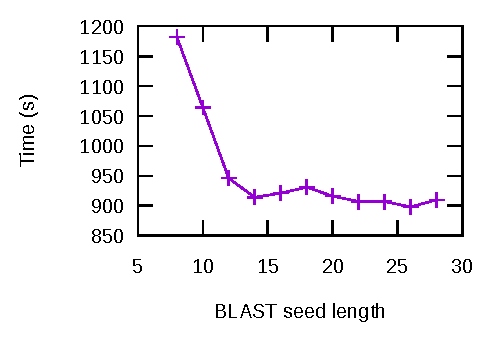
\includegraphics{img/time}
        \caption{Time needed by \acrshort{blast}--\blastobam{}.}
        \label{fig:time}
    \end{subfigure}
    \hfill
    \begin{subfigure}[b]{0.5\textwidth}
        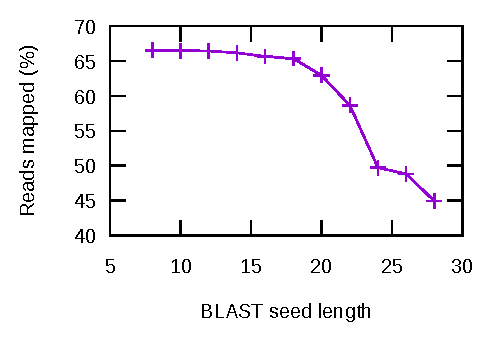
\includegraphics{img/nbReads}
        \caption{Percentage of reads mapped.}
        \label{fig:nbReads}
    \end{subfigure}
    \smallskip
    
    \begin{subfigure}[b]{0.5\textwidth}
        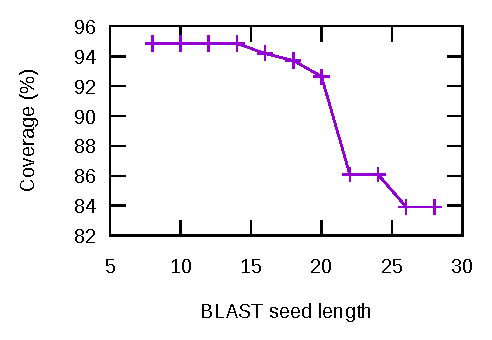
\includegraphics{img/coverage}
        \caption{Coverage.}
        \label{fig:coverage}
    \end{subfigure}
    \hfill
    \begin{subfigure}[b]{0.5\textwidth}
        \begin{flushright}
        \begin{minipage}[b]{0.75\textwidth}
        Results obtained with \gls{bwa}:
        \vspace{1.5ex}
        \begin{itemize}
            \item Time: 51 seconds
            \vspace{1.5ex}
            \item Reads mapped: 67.38\%
            \vspace{1.5ex}
            \item Coverage: 84.38\%
            \vspace{1.5ex}
        \end{itemize}
        \end{minipage}
        \end{flushright}
        \vspace{1.5cm}
        \caption{\acrshort{bwa} results}
        \label{fig:bwaResults}
    \end{subfigure}
    \caption[Results obtained with \acrshort{blast}--\blastobam{} and \acrshort{bwa}]{Results obtained with \acrshort{blast}--\blastobam{} (a,b,c) and \acrshort{bwa} (d).
    (a) Time needed by \acrshort{blast}--\blastobam{} to output the results. (b) Percentage of reads mapped. (c) Coverage. (a,b,c) are expressed as functions of \acrshort{blast} seed length.
    (d) \acrshort{bwa} results.}
    \label{fig:results}
\end{figure}

\begin{sidewaysfigure}
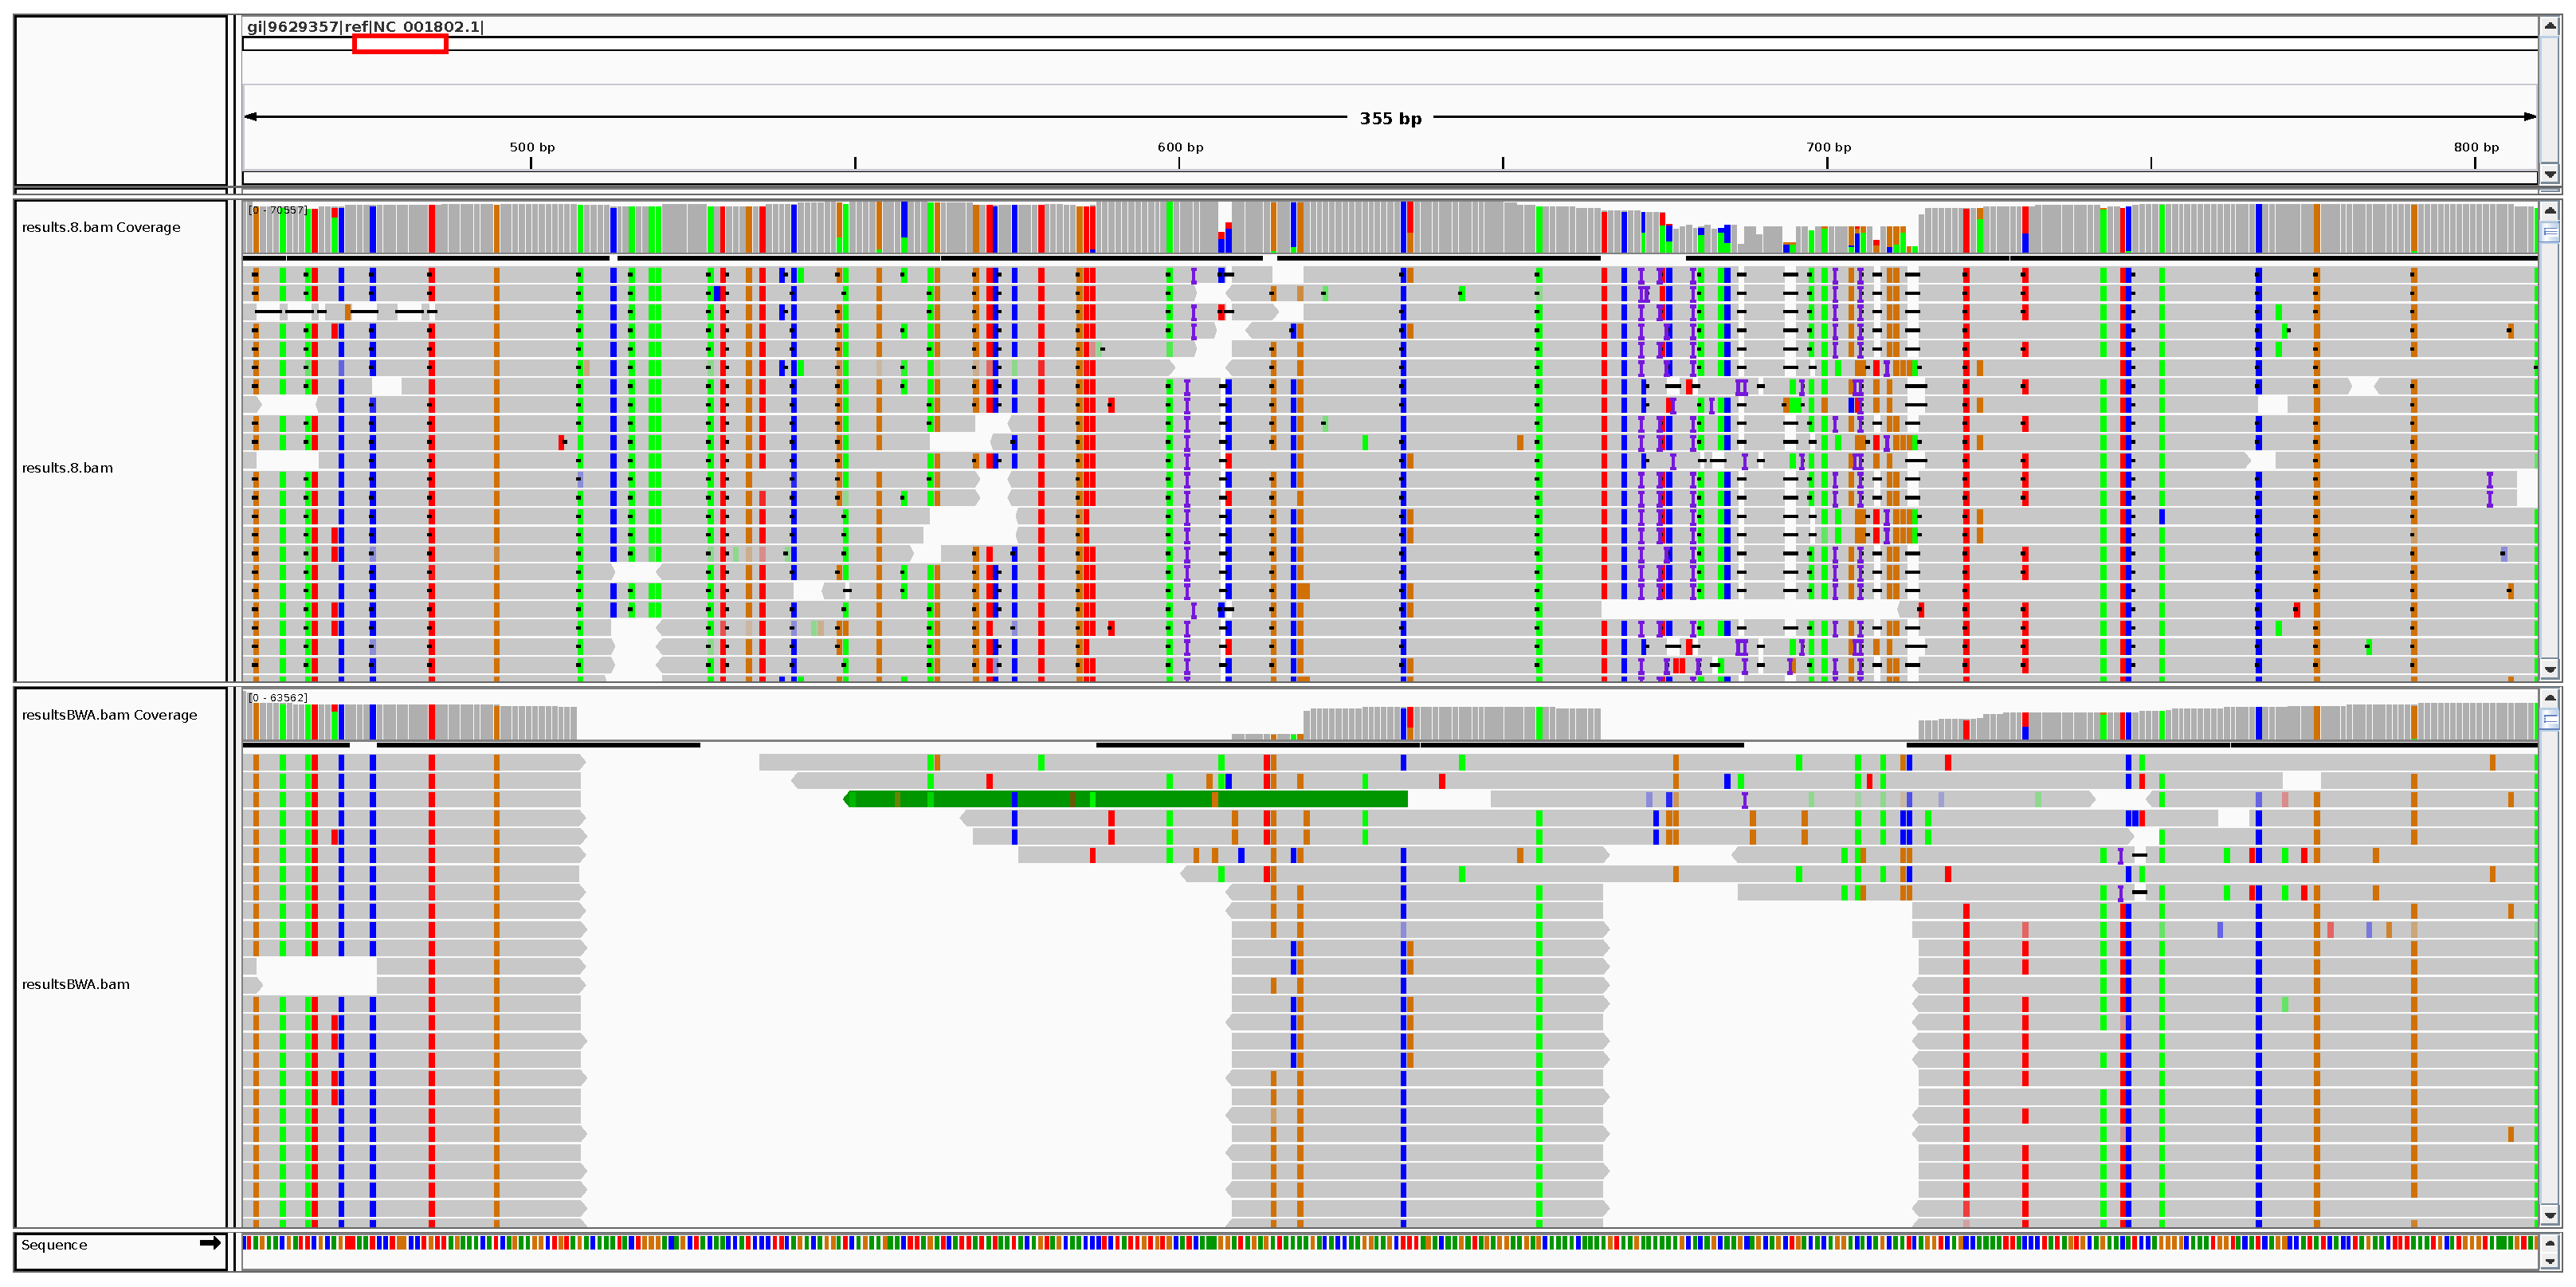
\includegraphics[scale=0.45]{img/igv01}
\caption[IGV representation of the alignments obtained with \acrshort{blast}--\blastobam{} and with \acrshort{bwa}.]
{IGV representation of the alignments obtained with \acrshort{blast}--\blastobam{} (\texttt{-word\_size~8}) and with \acrshort{bwa}. Upper part: \gls{blast}--\blastobam{}. Lower part: \gls{bwa}.}
\label{fig:igv}
\end{sidewaysfigure}
